\documentclass[fleqn, a4paper, 12pt, oneside]{amsart}
\usepackage{exsheets, tasks}
\usepackage{amsmath, amssymb, amsthm} %standard AMS packages
\usepackage{marginnote} %marginnotes
\usepackage{gensymb} %miscellaneous symbols
\usepackage{commath} %differential symbols
\usepackage{xcolor} %colours
\usepackage{cancel} %cancelling terms
\usepackage{siunitx} %formatting units
\usepackage{tikz, pgfplots} %diagrams
\usetikzlibrary{calc, hobby, patterns, intersections}
\usepackage{graphicx} %inserting graphics
\usepackage{hyperref} %hyperlinks
\usepackage{datetime} %date and time
\usepackage{ulem} %underline for \emph{}
\usepackage{xfrac} %inline fractions
\usepackage{enumerate} %numbered lists
\usepackage{float} %inserting floats
\usepackage{circuitikz} %circuit diagrams

\newcommand\numberthis{\addtocounter{equation}{1}\tag{\theequation}} %adds numbers to specific equations in non-numbered list of equations

\newcommand{\AxisRotator}[1][rotate=0]{
	\tikz [x=0.25cm,y=0.60cm,line width=.2ex,-stealth,#1] \draw (0,0) arc (-150:150:1 and 1);%
} %rotation symbols on axes

\theoremstyle{definition}
\newtheorem{example}{Example}
\newtheorem{definition}{Definition}

\theoremstyle{theorem}
\newtheorem{theorem}{Theorem}

\newcommand{\curl}{\mathrm{curl\,}}

\makeatletter
\@addtoreset{section}{part} %resets section numbers in new part
\makeatother

\renewcommand{\thesubsection}{(\arabic{subsection})}
\renewcommand{\thesection}{(\arabic{section})}

%section headings on left
\makeatletter
\def\specialsection{\@startsection{section}{1}%
	\z@{\linespacing\@plus\linespacing}{.5\linespacing}%
	%  {\normalfont\centering}}% DELETED
	{\normalfont}}% NEW
\def\section{\@startsection{section}{1}%
	\z@{.7\linespacing\@plus\linespacing}{.5\linespacing}%
	%  {\normalfont\scshape\centering}}% DELETED
	{\normalfont\scshape}}% NEW
\makeatother

%forces newline after subsection
\makeatletter
\def\subsection{\@startsection{subsection}{3}%
	\z@{.5\linespacing\@plus.7\linespacing}{.1\linespacing}%
	{\normalfont\itshape}}
\makeatother

\settasks{counter-format = tsk[1].}

\SetupExSheets{solution/print = true}

%opening
\title{Physics 2 : Assignment 2}
\author
{
	Aakash Jog\\
	ID : 989323563
}
\date{\formatdate{25}{3}{2015}}

\begin{document}
	
\maketitle
%\setlength{\mathindent}{0pt}

\begin{question}
	A charge $q$ sits at the back comer of a cube, as shown. What is the flux of $\overrightarrow{E}$ through the shaded side?
	\begin{figure}[H]
		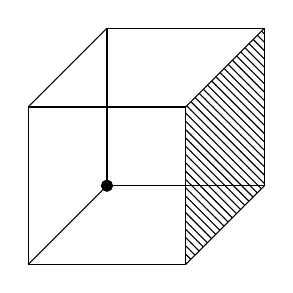
\begin{tikzpicture}
			\def\s{2};
		
			\draw (0,0) rectangle (\s,\s);
			\draw (1,1) rectangle ({\s + 1},{\s + 1});
			
			\draw 
				(0,0) -- ++(1,1)
				(0,\s) -- ++(1,1)
				(\s,0) -- ++(1,1)
				(\s,\s) -- ++(1,1);
				
			\filldraw (1,1) circle (2pt);
			
			\fill [pattern = north west lines] (\s,0) -- ++(0,\s) -- ++(1,1) -- ++(0,-\s) -- cycle;
		\end{tikzpicture}
	\end{figure}
\end{question}

\begin{solution}
	Let the area each surface of the box be $A$.\\
	If the charge was kept in the centre of a box with faces of area $4A$, the total flux through all surfaces, i.e. through $24 A$ will be $\oint \overrightarrow{E} \dif \overrightarrow{A}$.\\
	Therefore, the flux through the shaded area is 
	\begin{align*}
		\phi &= \dfrac{1}{24} \oint \overrightarrow{E} \dif \overrightarrow{A}\\
		&= \dfrac{1}{24} \dfrac{q}{\varepsilon_0}
	\end{align*}
\end{solution}

\begin{question}
	Find the electric field a distance $s$ from an infinitely long straight wire, which carries a uniform line charge $\lambda$.
\end{question}

\begin{solution}
	Consider a cylindrical Gaussian surface, with radius $r$ and length $L$ such that the wire passes through its axis.\\
	Therefore, by Gauss' Law,
	\begin{align*}
		\oint \overrightarrow{E} \cdot \dif \overrightarrow{A} &= \dfrac{q_{\textnormal{inside}}}{\varepsilon_0}\\
		\therefore E (2 \pi r L) &= \dfrac{\lambda L}{\varepsilon_0}\\
		\therefore E &= \dfrac{\lambda}{2 \pi \varepsilon_0 r}
	\end{align*}
\end{solution}

\begin{question}
	Find the electric field inside a sphere which carries a charge density proportional to the distance from the origin, $\rho = kr$, for some constant $k$.
\end{question}

\begin{solution}
	\begin{figure}[H]
		\begin{tikzpicture}
			\def\R{3};
			\def\r{2};
		
			\draw (0,0) circle (\R);
			
			\draw [dashed] (0,0) circle (\r);
		\end{tikzpicture}
	\end{figure}
	Consider a spherical Gaussian surface of radius $a$ as shown.\\
	The charge inside the Gaussian surface is
	\begin{align*}
		q_{\textnormal{inside}} &= \int\limits_{0}^{a} \rho \cdot 4 \pi r^2 \dif r\\
		&= \int\limits_{0}^{a} 4 \pi k r^3 \dif r\\
		&= \left. \pi k r^4 \right|_{0}^{a}\\
		&= \pi k a^4
	\end{align*}
	Therefore, by Gauss' Law,
	\begin{align*}
		\oint \overrightarrow{E} \cdot \dif \overrightarrow{A} &= \dfrac{q_{\textnormal{inside}}}{\varepsilon_0}\\
		\therefore E (4 \pi a^2) &= \dfrac{\pi k a^4}{\varepsilon_0}\\
		\therefore E &= \dfrac{k a^2}{4 \varepsilon_0}
	\end{align*}
\end{solution}

\begin{question}
	A hollow spherical shell carries charge density $\rho = \dfrac{k}{r^2}$ in the region $a \le r \le b$. Find the electric field in three regions:
	\begin{enumerate}[(i)]
		\item $r < a$
		\item $a < r < b$
		\item $b < r$
	\end{enumerate}
	Plot $|E|$ as a function of $r$.
\end{question}

\begin{solution}
	\begin{figure}[H]
		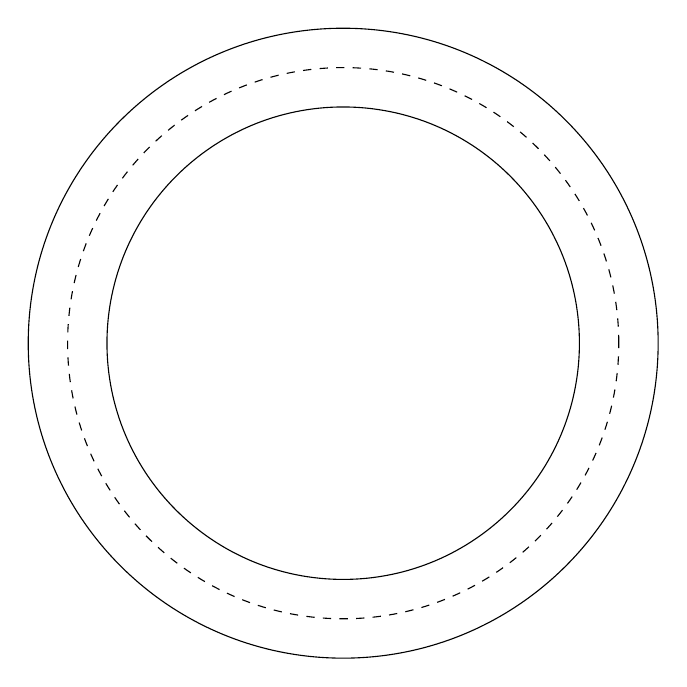
\begin{tikzpicture}
			\def\a{3};
			\def\b{4};
			\def\r{3.5};
			
			\draw (0,0) circle (\a);
			\draw (0,0) circle (\b);
			
			\draw [dashed] (0,0) circle (\r);
		\end{tikzpicture}
	\end{figure}
	Consider a spherical Gaussian surface of radius $r$.\\
	~\\
	If $r < a$, the total charge inside the Gaussian surface is zero.
	Therefore, by Gauss' Law,
	\begin{align*}
		E (4 \pi r^2) &= \dfrac{0}{\varepsilon_0}\\
		\therefore E &= 0
	\end{align*}
	~\\
	If $a < r < b$,
	\begin{align*}
		q_{\textnormal{inside}} &= \int\limits_{a}^{r} \rho \cdot 4 \pi {\tilde{r}}^2 \dif \tilde{r}\\
		&= \int\limits_{a}^{r} \dfrac{k}{{\tilde{r}}^2} \cdot 4 \pi {\tilde{r}}^2 \dif \tilde{r}\\
		&= \int\limits_{a}^{r} 4 k \pi \dif \tilde{r}\\
		&= 4 k \pi (r - a)
	\end{align*}
	Therefore, by Gauss' Law,
	\begin{align*}
		E (4 \pi r^2) &= \dfrac{4 k \pi (r - a)}{\varepsilon_0}\\
		\therefore E &= \dfrac{k (r - a)}{\varepsilon_0 r^2}
	\end{align*}
	~\\
	If $b < r$,
	\begin{align*}
		q_{\textnormal{inside}} &= 4 k \pi (b - a)
	\end{align*}
	Therefore, by Gauss' Law,
	\begin{align*}
		E (4 \pi r^2) &= \dfrac{4 k \pi (b - a)}{\varepsilon_0}\\
		\therefore E &= \dfrac{k (b - a)}{\varepsilon_0 r^2}
	\end{align*}
	~\\
	\begin{figure}[H]
		\begin{tikzpicture}
			\begin{scope}[gray, -stealth]
				\draw (0,0) -- (6,0) node [right] {$r$};
				\draw (0,0) -- (0,4) node [above] {$|E|$};
			\end{scope}
			
			\draw (0,0) -- (1,0) to [out = 80, in = 180] (3,2) to [out = -90, in = 180] (5,0);
			
			\fill (1,0) circle (1pt) node [below] {$a$};
			\fill (3,0) circle (1pt) node [below] {$b$};
		\end{tikzpicture}
	\end{figure}
\end{solution}

\begin{question}
	A long coaxial cable carries a uniform volume charge density $\rho$ on the inner cylinder (radius $a$), and a uniform surface charge density on the outer cylindrical shell (radius $b$). This surface charge is negative and of just the right magnitude so that the cable as a whole is electrically neutral. Find the electric field in each of the three regions:
	\begin{enumerate}[(i)]
		\item inside the inner cylinder $(s < a)$
		\item between the cylinders$ (a < s < b)$
		\item outside the cable $(b < s)$
		Plot $|E|$ as a function of $s$.
	\end{enumerate}
\end{question}

\begin{solution}
	Consider a cylindrical Gaussian surface with radius $s$ and length $L$, concentric to the cable.\\
	~\\
	If $s < a$,
	\begin{align*}
		q_{\textnormal{inside}} &= \rho \cdot \pi s^2 L
	\end{align*}
	Therefore, by Gauss' Law,
	\begin{align*}
		E (2 \pi s L) &= \dfrac{\pi \rho s^2 L}{\varepsilon_0}\\
		\therefore E &= \dfrac{\rho s}{2 \varepsilon_0}
	\end{align*}
	~\\
	If $a < s < b$,
	\begin{align*}
		q_{\textnormal{inside}} &= \rho \cdot \pi a^2 L
	\end{align*}
	Therefore, by Gauss' Law,
	\begin{align*}
		E (2 \pi s L) &= \dfrac{\pi \rho a^2 L}{\varepsilon_0}\\
		\therefore E &= \dfrac{\rho a^2}{2 s \varepsilon_0}
	\end{align*}
	~\\
	If $b < s$,
	\begin{align*}
		q_{\textnormal{inside}} &= 0
	\end{align*}
	Therefore, by Gauss' Law, 
	\begin{align*}
		E &= 0
	\end{align*}
	\begin{figure}[H]
		\begin{tikzpicture}
			\begin{scope}[gray, -stealth]
			\draw (0,0) -- (6,0) node [right] {$r$};
			\draw (0,0) -- (0,4) node [above] {$|E|$};
			\end{scope}
			
			\draw (0,0) -- (2,2) to [out = -90, in = 180] (3,1);
			\draw (3,0) -- (5,0);
			
			\fill (2,0) circle (1pt) node [below] {$a$};
			\fill (3,0) circle (1pt) node [below] {$b$};
		\end{tikzpicture}
	\end{figure}
\end{solution}

\begin{question}
	An infinite plane slab, of thickness $2d$, carries a uniform volume charge density $\rho$. Find the electric field, as a function of $y$, where $y = 0$ at the centre. Plot $\overrightarrow{E}$ versus $y$, calling $E$ positive when it points in the positive $+y$ direction and negative when it points in the $-y$ direction.
\end{question}

\begin{solution}
	Consider a cylindrical Gaussian surface with base area $A$, as shown.
	\begin{figure}[H]
		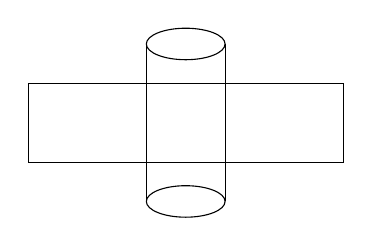
\begin{tikzpicture}
			\def\d{0.5};
			\def\l{4};
			\def\r{0.5};
			
			\draw (-\l/2,-\d) rectangle (\l/2,\d);
			
			\draw (0,{\d + 0.5}) circle [x radius = \r, y radius = 0.4*\r];
			\draw (0,{-\d - 0.5}) circle [x radius = \r, y radius = 0.4*\r];
			
			\draw (-\r,{\d + 0.5}) -- (-\r,{-\d - 0.5});
			\draw (\r,{\d + 0.5}) -- (\r,{-\d - 0.5});
		\end{tikzpicture}
	\end{figure}
	If $|y| < d$,
	\begin{align*}
		q_{\textnormal{inside}} &= \rho \cdot 2 y A
	\end{align*}
	Therefore, by Gauss' Law,
	\begin{align*}
		E \cdot 2A &= \dfrac{2 \rho y A}{\varepsilon_0}\\
		\therefore E &= \dfrac{\rho y}{\varepsilon_0}
	\end{align*}
	~\\
	If $|y| > d$,
	\begin{align*}
		q_{\textnormal{inside}} &= \rho \cdot 2d A
	\end{align*}
	Therefore, by Gauss' Law, 
	\begin{align*}
		E \cdot 2A &= \dfrac{2 \rho A d}{\varepsilon_0}\\
		\therefore E &= \dfrac{\rho d}{\varepsilon_0}
	\end{align*}
	\begin{figure}[H]
		\begin{tikzpicture}
			\begin{scope}[-stealth]
			\draw (-5,0) -- (5,0) node [right] {$|r|$};
			\draw (0,-3) -- (0,3) node [above] {$\overrightarrow{E}$};
			\end{scope}
			
			\draw (0,0) -- (2,2) -- (4,2);
			\draw (-4,-2) -- (-2,-2) -- (0,0);
			
			\fill (2,0) circle (1pt) node [below] {$d$};
			\fill (-2,0) circle (1pt) node [below] {$-d$};
		\end{tikzpicture}
	\end{figure}
\end{solution}

\end{document}